\sekshun{Numerical Integration}
\label{Numerical_Integration}
\index{numerical integration}

\section{Rectangle Method}
The rectangle method computes an approximation to a 
definite integral by finding the area of a collection of rectangles whose heights are determined 
by the values of the function.  Specifically, the interval $[a,b]$ over which the function is to 
be integrated is divided into $N$ equal subintervals of length $h = (b-a)/N$. The rectangles are 
drawn with one base along the $x$-axis. Depending on whether the method is left, right, or midpoint,
the left corner, right corner, or midpoint, respectively, of the side opposite the base lies on the 
graph of the function. The approximation to the integral is 
then calculated by adding up the areas (base multiplied by height) of the $N$ rectangles, giving the formula:
\begin{equation}
\int_a^b f(x) dx \approx h \sum_{n=0}^{N-1} f(x_n) \label{eq:rectangle}
\end{equation}
where
\begin{equation}
h=(b-a)/N 
\end{equation}

\begin{table}
\centering
\caption{Formula for $x_n$ in Equation \ref{eq:rectangle} of rectangle numerical integration methods.}
\label{tab:xn-rectangle}
\begin{tabular}{cc}\\
Rectangle Method & $x_n$ \\ \toprule
left & $a+nh$ \\ \midrule
right & $a+(n+1)h$ \\ \midrule
midpoint & $a+\left(n + \frac{1}{2}\right)h$ \\ \bottomrule
\end{tabular}
\end{table}

The formula for $x_n$ for the left, right, and midpoint methods are given in Table \ref{tab:xn-rectangle}.
As $N$ gets larger, the rectangle method becomes more accurate. This is illustrated in the series of plots
in Figure \ref{fig:rectangle}.

\begin{figure}
\centering
\subcaptionbox{$N=4$}{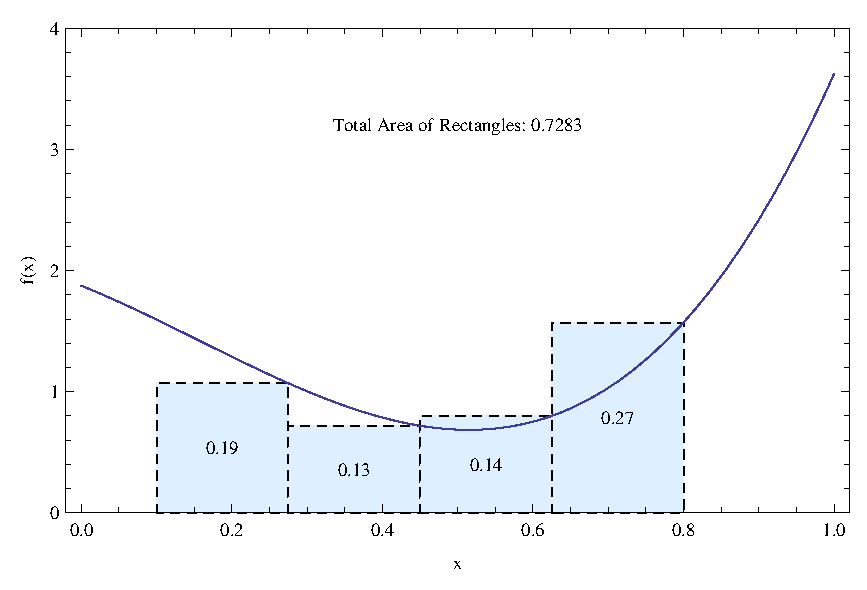
\includegraphics[scale=.6]{fig/rightrectangle-4.eps}}
\subcaptionbox{$N=6$}{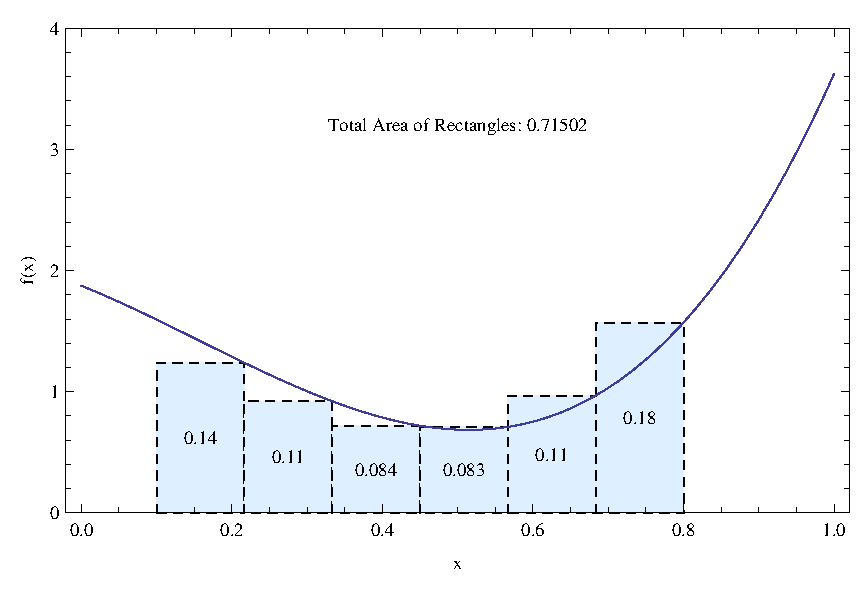
\includegraphics[scale=.6]{fig/rightrectangle-6.eps}}
\subcaptionbox{$N=10$}{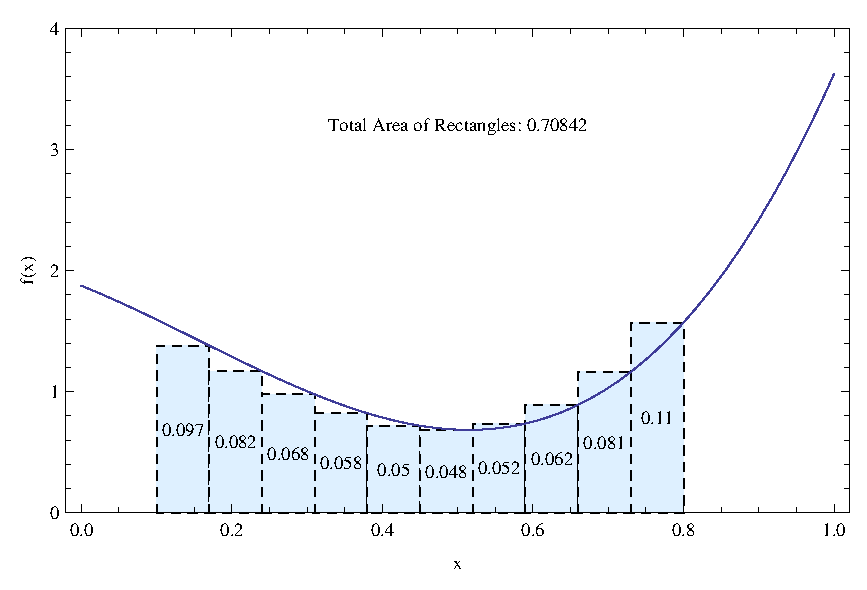
\includegraphics[scale=.6]{fig/rightrectangle-10.eps}}
\caption{Numerical integration of $f(x) = (2 x-0.5)^3+(1.5 x-1)^2-x+1$ for $x$ in $[0.1,0.8]$
by the (right) rectangle method for increasing values of $N$. The number inside each rectangle is
the area of that rectangle, and the total area is displayed on each graph.
The exact value of the integral is 0.70525.}\label{fig:rectangle}
\end{figure}

If $f(x)$ is increasing or decreasing on the interval $[a,b]$, the maximum error $E$ 
for left or right rectangular numerical integration is given by
\begin{equation}
E \leq \frac{b-a}{N}\left|f(b)-f(a)\right| \label{eq:lr-rectangle-max-error}
\end{equation}

\begin{enumspec}
\item\spec{1}
Using Create a helper function to compute the maximum error: \meetsrequirement{5}
\end{enumspec}

\begin{chapelhelper}{leftRightRectangleIntegrationMaximumError.chpl}
\begin{chapel}
proc leftRightRectangleIntegrationMaximumError(a: real, b: real, N: int, f){
  return ((b-a)/N)*abs(f(b)-f(a));
}
\end{chapel}
\end{chapelhelper}

\begin{enumspec}
\item\spec{2}
Testing for $f(x) = x^3$, with $a=0$, $b=1$, and $N=100$.
Since the function is increasing on the interval $[0,1]$, 
the maximum error given by equation \ref{eq:lr-rectangle-max-error} is 0.01.  \meetsrequirement{5.1}
\end{enumspec}

\begin{chapelexample}{leftRectangleIntegrationTest.chpl}
A test for \lstinline{leftRectangleIntegration}:
\begin{chapelpre}
use leftRightRectangleIntegrationMaximumError;
use leftRectangleIntegration;
\end{chapelpre}
\begin{chapel}
proc f(x:real):real {
  return x**3;
} 
  
var calculated:real;
var exact:real = 0.25;  // from Mathematica
var maximumError:real = leftRightRectangleIntegrationMaximumError(0.0,1.0,100,f);
var verified:bool;

calculated = leftRectangleIntegration(a = 0.0, b = 1.0, N = 100, f = f);
verified = (abs(calculated - exact) <= maximumError);
writeln(verified);
\end{chapel}
enter some text here...
\begin{chapelpost}
\end{chapelpost}
\begin{chapeloutput}
true
\end{chapeloutput}
\end{chapelexample}

The code that provides the \lstinline{leftRectangleIntegration} function is straightforward:
\begin{chapelsource}{leftRectangleIntegration.chpl}
\begin{chapel}
proc leftRectangleIntegration(a: real(64), b: real(64), N: int(64), f): real(64){
  var h: real(64) = (b - a)/N;
  var sum: real(64) = 0.0;
  var x: real(64);
  for n in 0..N-1 {
    x = a + n * (b-a)/N;
    sum = sum + f(x);
  }
  return h * sum;
}
\end{chapel}
\end{chapelsource}

For a function $f$ which is twice differentiable, the maximum error $E$ is given by
the following equation:
\begin{equation}
E \leq \frac{(b-a)h^2}{24} f''(\xi) \label{eq:rectangle-max-error}
\end{equation}
for some $\xi$ in $[a,b]$.

Create a helper function to compute the maximum error:
\begin{chapelhelper}{midpointRectangularIntegrationMaximumError.chpl}
\begin{chapel}
proc midpointRectangularIntegrationMaximumError(a: real, b: real, N: int, fppxi){
  var h:real = (b-a)/N;
  return ((b-a)*h**2/24) * fppxi;
}
\end{chapel}
\end{chapelhelper}
